\documentclass{TDP005mall}

\usepackage{mathtools}
\usepackage{float}

\newcommand{\version}{Version 1.0}
\author{David Dumminsek, \url{davdu153@student.liu.se}\\
  Haris Basic, \url{harba466@student.liu.se}\\}
\title{Designspecifikation}
\date{2022-11-25}
\rhead{David Dumminsek\\
Haris Basic\\}



\begin{document}
\projectpage
\section{Revisionshistorik}
\begin{table}[!h]
\begin{tabularx}{\linewidth}{|l|X|l|}
\hline
Ver. & Revisionsbeskrivning & Datum \\\hline
  1.0 & Skrev diskussion, UML och externfilformat. Första utkast slutfört och inlämnat & 2022-11-25\\\hline
\end{tabularx}
\end{table}


\section{Klasser}
Vilka klasser som kommer användas i spelet.

\subsection{Player}
Denna klass ska modellera spelaren.
Det ska vara möjligt för spelaren att röra sig, kollidera och skjuta projektiler.
\subsubsection*{Klassrelationer}
\begin{enumerate}
  \item \textbf{Projectile:} Player använder ett projectile objekt för att beskriva hur spelarens projektil fungerar.\\
                    Om spelaren delar koordinater med en projektil så dör spelaren.
  \item \textbf{Enemy:} Om spelaren delar koordinater med ett Enemy objekt dör spelaren.
  \item \textbf{Game:} Vart Player objektet skapas.
\end{enumerate}
\subsubsection*{Konstruktorer}
\begin{enumerate}
  \item \textbf{Player()} Sätter \textbf{life} (spelarens liv) till 2, \textbf{speed} (spelarens rörelsehastighet) till 0.1 och koordinaterna till det som är mitt i botten. Samt så konstrueras ett Projectile objekt.
  \item \textbf{Player(Projectile a):} Är lik default constructorn utom att ett valfri Projectile objekt kan användas.
    \item \textbf{Player(const\& Enemy) = default} Copy constructor
  \item \textbf{Player(const\&\& Enemy) = default} Move constructor
\end{enumerate}
\subsubsection*{Variabler}
\begin{enumerate}
  \item \textbf{int x{}:} x-koordinater för spelaren
  \item \textbf{int y{}:} y-koordinater för spelaren
  \item \textbf{float speed{}:} hur många x och/eller y koordinater spelaren rör sig per tick.
  %\item \textbf{int point:} hur många poäng spelaren har
  \item \textbf{int life{}:} hur många liv spelaren har.
  \item \textbf{Projectile pro{}:} Projectile objekt som beskriver hur projektilen rör sig och hur mycket skada den gör:
\end{enumerate}
\subsubsection*{Funktioner}
\begin{enumerate}
  \item \textbf{Enemy\& operator=(const\& Enemy rhs) = default:} Copy constructor
  \item \textbf{Enemy\& operator=(Enemy\&\& rhs) = default:} Move constructor
  \item \textbf{~Enemy():} Destructor
  \item \textbf{void move():} Tar emot användarinmatning från game loopet och uppdaterar koordinaterna med \textbf{speed} variablen.
    Om koordinaterna skulle hamna utanför spelet så ändras inte koordinaterna (kollidering med fiende kommer hanteras i \textbf{Game} klassen). 
  \item \textbf{void shoot():} Skapar \textbf{Projectile} objekt som startar med \textbf{Player} (spelarens) koordinater och rör sig rakt fram i en hastighet beroende på objektet. 
  \item \textbf{void die():} Ändrar koordinaterna till de ursprungliga koordinaterna och minskar \textbf{life} med 1 (life - 1).
  
\end{enumerate}
\subsection{Game}
Denna klass tar hand om funktionerna som används i gameloopet:
Klassen ska huvudsakligen rendera och updatera.
\subsubsection*{Klassrelationer}
\begin{enumerate}
  \item \textbf{Projectile: } Håller koll på koordinaterna för alla projektiler
  \item \textbf{Player: } Håller koll på spelarens koordinater.
  \item \textbf{Enemy: } Håller koll på alla fientliga enheters koordinater.
 \end{enumerate}
 \subsubsection*{Konstruktorer}
 \begin{enumerate}
   \item \textbf{Game():} Läser alla level filer (spelets banor) och lägger det i \textbf{level} vektorn. 
                          Skapar \textbf{Player} objektet.
 \end{enumerate}
 \subsubsection*{Variabler}
 \begin{enumerate}
   \item \textbf{vector<map> level:} En vektor av \textbf{map} typen som innehåller bl.a när fiender skapas och värden för att konstruera ett \textbf{Enemy} objekt.
   \item \textbf{int tick:} En integer som updateras efter varje gameloop och används för att bestämma när fiender skapas, var de befinner sig beroende på deras rörelse funktion och när spelaren har nått slutet av banan.
    \item \textbf{vector<Enemy> enemies: } En vektor med alla fiende objekt.
    \item \textbf{vector<Projectile> enemyProjectile} En vektor med alla projektiler från fiender.
    \item \textbf{vector<Projectile> playerProjectile} En vektor med alla projektiler från spelaren.
 \end{enumerate}
 \subsubsection*{Funktioner}
 \begin{enumerate}
   \item \textbf{void collisionCheck(): } Jämför alla koordinater för fiender samt deras projektiler med spelarens koordinater.
                                          Om koordinaterna är tillräckligt nära varandra så kallas \textbf{Player.die()} funktionen.
                                          Jämför även koordinaterna för spelarens projektiler med fiendernas koordinater. Om spelarens projektiler är tillräckligt nära en fiende så kallas \textbf{Enemy.takeDmg()} funktionen.
  \item \textbf{void update(): } Ändrar koordinater för spelaren och fiender med deras \textbf{move()} funktioner.
                                Kallar också \textbf{spawnEnemy()}, \textbf{updateProjectile}, \textbf{collisionCheck} och \textbf{victory}.
  \item \textbf{void render(): } Renderar spelaren och alla fiender och projektiler.
  \item \textbf{void victory(): } Kollar om \textbf{tic} är över en viss gräns och om alla fiender har eliminerats. Om det stämmer så startas nästa bana.
  \item \textbf{void spawnEnemy(): } Kollar nuvarande \textbf{map} variabel i \textbf{level} vektorn om \textbf{tick} är lika med \textbf{tickSpawn}.
                                      Om det är det så skapas ett \textbf{Enemy} objekt med hjälp av alla \textbf{map} värden.

  \item \textbf{void updateProjectile(): } Går igenom varje \textbf{Enemy} objekt och kallar deras \textbf{shoot()} funktion för att skapa \textbf{Projectile} objekt.
                                           Lägger till nya skapade projektiler i \textbf{enemyProjectile} variablen.
                                           Uppdaterar koordinaterna på alla projektiler med hjälp av \textbf{Projectile.move()} funktionen.

  \end{enumerate}
  
\vspace{3cm}  
  
\section{Diskussion}

De främsta fördelarna med vår design är att det är lätt att bygga upp en grund för spelet rent kodmässigt samt att det är lätt att läsa av klasser på ett överskådligt sätt. Resultatet av detta är att det går att se hur allting fungerar på ett enkelt och översiktligt sätt. En positiv effekt av vår design är att filuppdelning blir lättare, vilket i sin tur gör att även kompilering blir betydligt lättare.

Det finns dock ett flertal nackdelar med vår design. Om någonting skulle gå fel vid utvecklandet av spelet så blir det svårt att fastställa exakt var en ändring behöver göras eftersom varje klass innehåller många olika delar. Ännu en nackdel är att om vi vill ändra på en funktion som är lik en funktion i en annan klass så måste vi göra den ändringen i alla liknande klasser (eftersom att vi ej använder polymorfi). 

Om vi exempelvis skulle göra en ändring i en move-funktion så behöver vi även göra ändringar hos andra move-funktioner då de är uppbyggda på ett liknande sätt. Ytterligare problem med vår design är att det är svårt att hålla koll på alla olika funktioner (eftersom att det finns väldigt många olika) och om vi i framtiden skulle behöva dela upp klasser i flera klasser så kommer det bli en väldigt rörig och tidskrävande process.

Det finns väldigt mycket upprepning i vår kod eftersom att vi inte använder oss av polymorfi. Ett sätt vi skulle kunna ha gjort saker och ting annorlunda är att vi exempelvis skulle kunna ha använt polymorfi till allt som rör på sig. 

Ett exempel på vad man skulle kunna ha gjort är att göra så att det fanns en överklass till de som de ärver datamedlemmar av funktioner ifrån. Detta hade gjort det betydligt enklare att fastställa var ett potentiellt fel har skett samt göra det enklare att göra ändringar i koden utan att behöva göra ändringar i alla liknande klasser. Användning av polymorfi hade minskat mängden upprepning i vår kod, vilket skulle göra den ännu mer läsbar och enklare att tyda och förstå. Det hade blivit enklare att hålla koll på alla olika funktioner. 

\section{Externfilformat}
Tar användning av en json fil för att bestämma när fiender skapas, hur de rör sig och hur deras projektiler rör sig.
Denna fil används alltså för att bygga upp en bana med att konstruera fiender vid specifika tider och positioner.
Själva jsonfilen är uppbyggd av en json array med olika json objekt. I dessa json objekt finns det 7 olika variabler, dessa är:
\begin{enumerate}
  \item \textbf{id}: Ett unikt nummer för varje fiende
  \item \textbf{tickSpawn}: Vid vilken tick fienden ska skapas (måste vara sorterad, där minsta är högst upp)
  \item \textbf{x}: x-koordinat där fienden ska skapas
  \item \textbf{y}: y-koordinat där fienden ska skapas
  \item \textbf{spd}: Hur många y koordinater fiender rör sig på en tick
  \item \textbf{movement}: Ett json objekt som beskriver en polynomfunktion, används för rörelsemönster för fienden
  \item \textbf{projectile}: Ett json objekt som beskriver en polynomfunktion, används för rörelsemönstret för projektilerna fienden skjuter
\end{enumerate}

\vspace{3cm}

\subsection{Rörelse}
En polynom av den fjärde graden används för att simulerara rörelsen för fiender och projektiler.
Som ett json objekt beskrivs funktionen som följande:\\

\begin{figure}[H]
  \begin{center}
    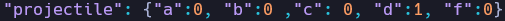
\includegraphics[width=0.6\textwidth]{poly.png}
  \end{center}
  \caption{Json objekt som beskriver en polynom funktion}
  \label{fig:}
\end{figure}
Alla variabler i Json objectet är då konstanterna i polynomfunktionen. Just i figur 1 så beskriver json objektet en projektil som åker snedd längst skärmen. 
Det json objektet beskriver alltså funktionen: 
\begin{figure}[H]
  \begin{center}
    $$y = x$$
  \end{center}
  \caption{Enkel linjär funktion}
  \label{fig:}
\end{figure}
\begin{figure}[H]
  \begin{center}
    $$ ax^4 + bx^3 + cx^2 + dx + f $$
  \end{center}
  \caption{Polynom av fjärde graden}
  \label{fig:}
\end{figure}

\vspace{10cm}

\section{UML Klass Diagram}
Klassdiagrammet för spelet:
\begin{figure}[H]
  \begin{center}
    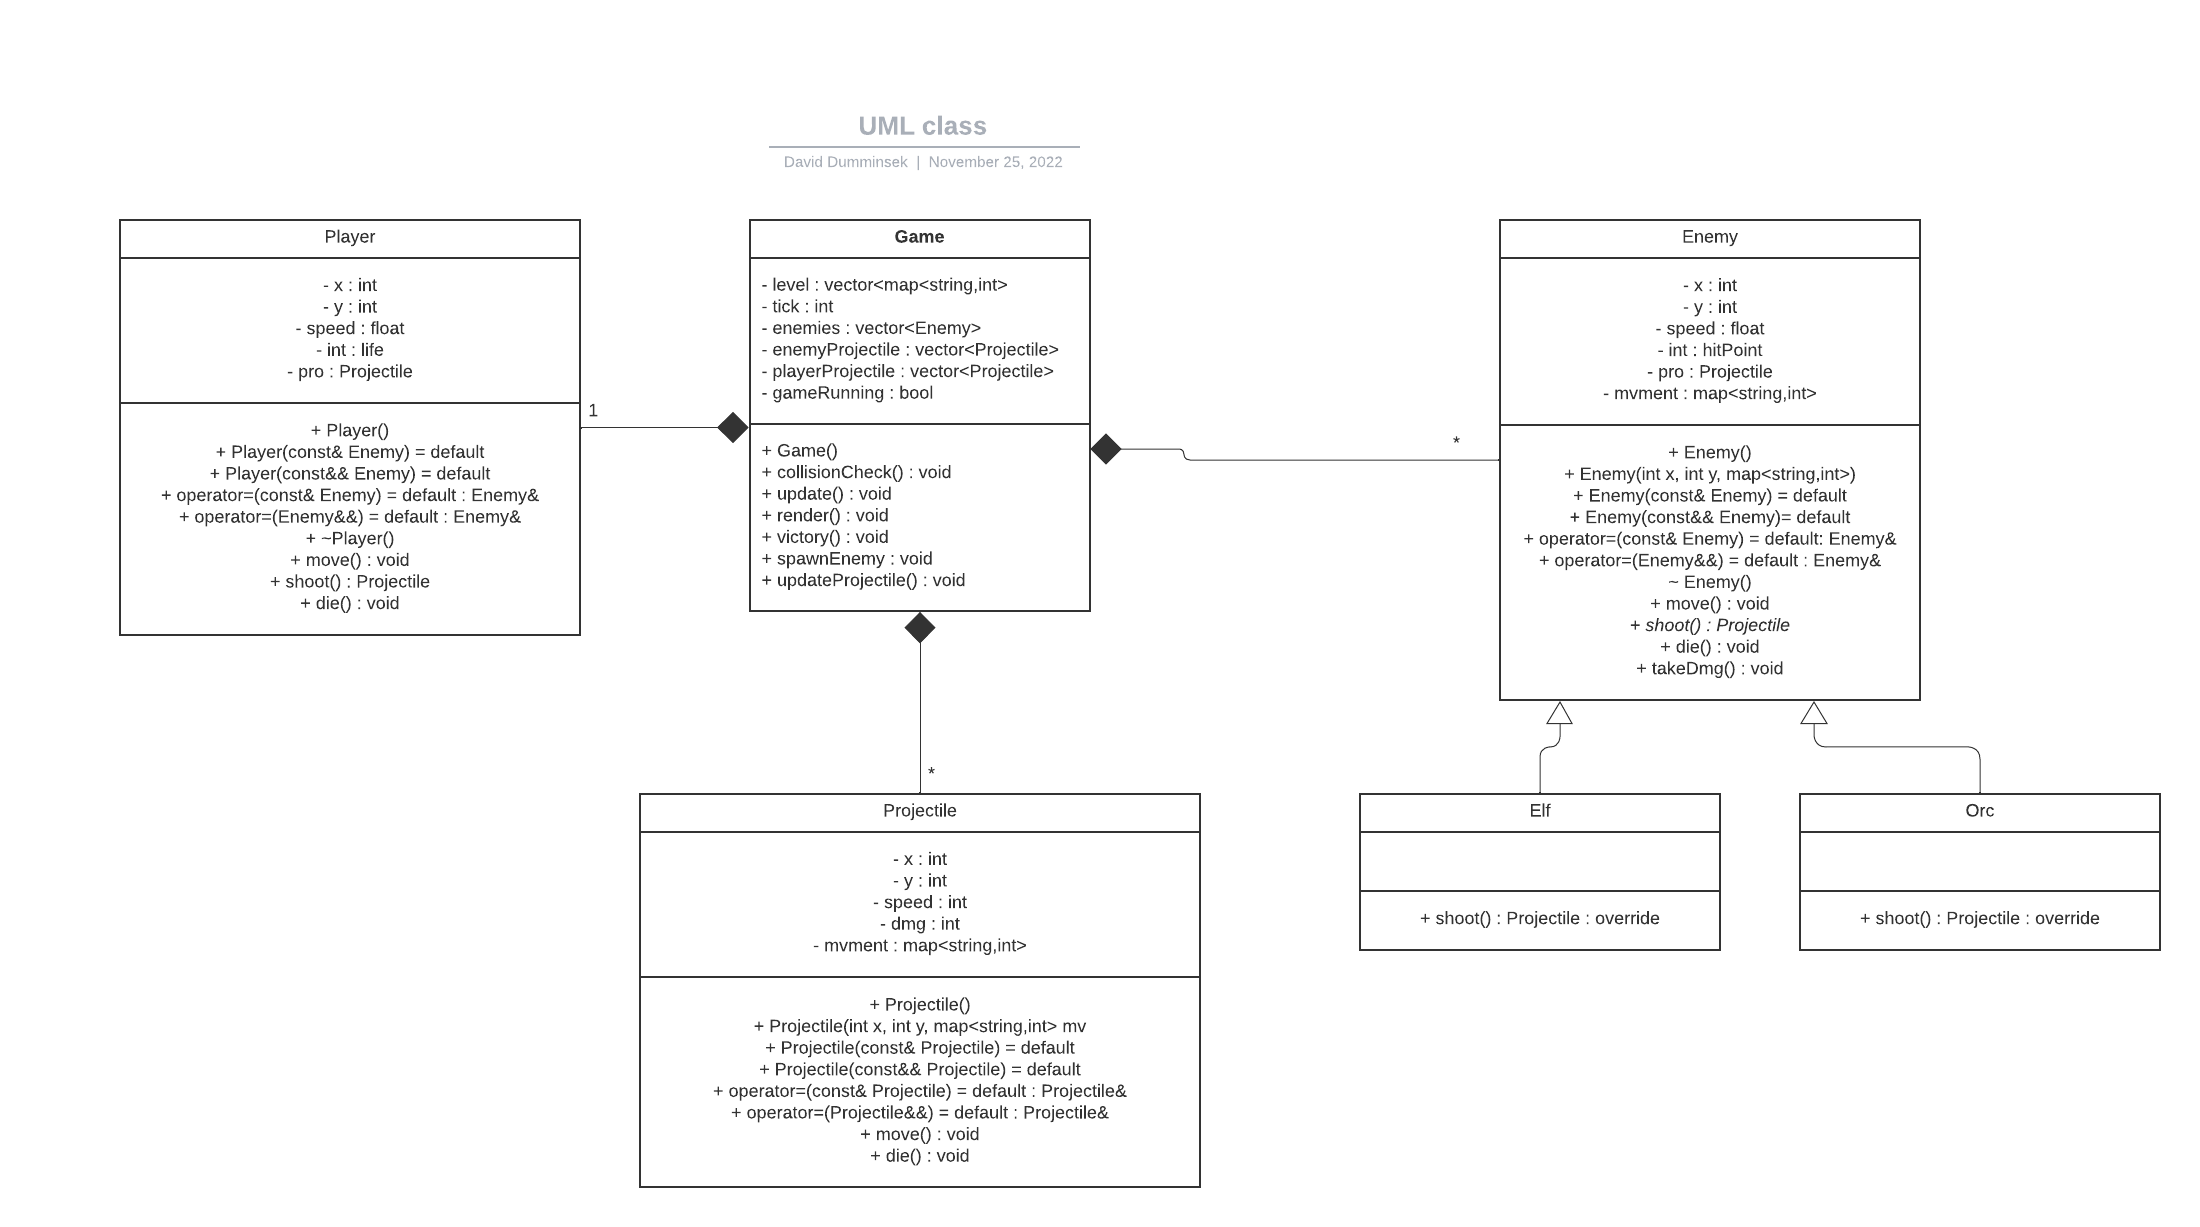
\includegraphics[width=0.95\textwidth]{UML class.png}
  \end{center}
  \caption{}
  \label{fig:}
\end{figure}




\end{document}
